\documentclass[../../main.tex]{subfiles}
\graphicspath{{../../image/}{../../figure/}}
\begin{document}

\section{真非线性系统中的波相互作用}\label{section:ch13-真非线性波相互作用}

我们现踏上漫长的征程，它最终将导向稳定性估计\eqref{align:ch13-h-sup}、\eqref{align:ch13-h-tv}与\eqref{align:ch13-h-lip}。第一步是估计近似解 $U_h$ 的总变差的局部变化。为简单起见，我们把讨论限于特征族要么真非线性、要么线性退化的系统。
一般情形远为复杂，将在\cref{section:ch13-一般系统}中扼要讨论。

按构造格式，从网格点 $(x_{r-1},t_{s-1})$（$r+s$ 为偶数）发出的波扇的一部分，与从网格点 $(x_{r+1},t_{s-1})$ 发出的波扇的一部分相结合，产生从网格点 $(x_r,t_s)$ 发出的波扇。把网格点 $(x_r,t_s)$ 围在一个菱形区域 $\Delta_s^r$ 中可方便地说明这一点，该菱形的四个顶点为周围的四个采样点 $(y_s^{r-1},t_s)$、$(y_{s-1}^r,t_{s-1})$、$(y_s^{r+1},t_s)$ 与 $(y_{s+1}^r,t_{s+1})$；见\cref{figure:ch13-菱形相互作用}。

\begin{figure}[ht]
\centering
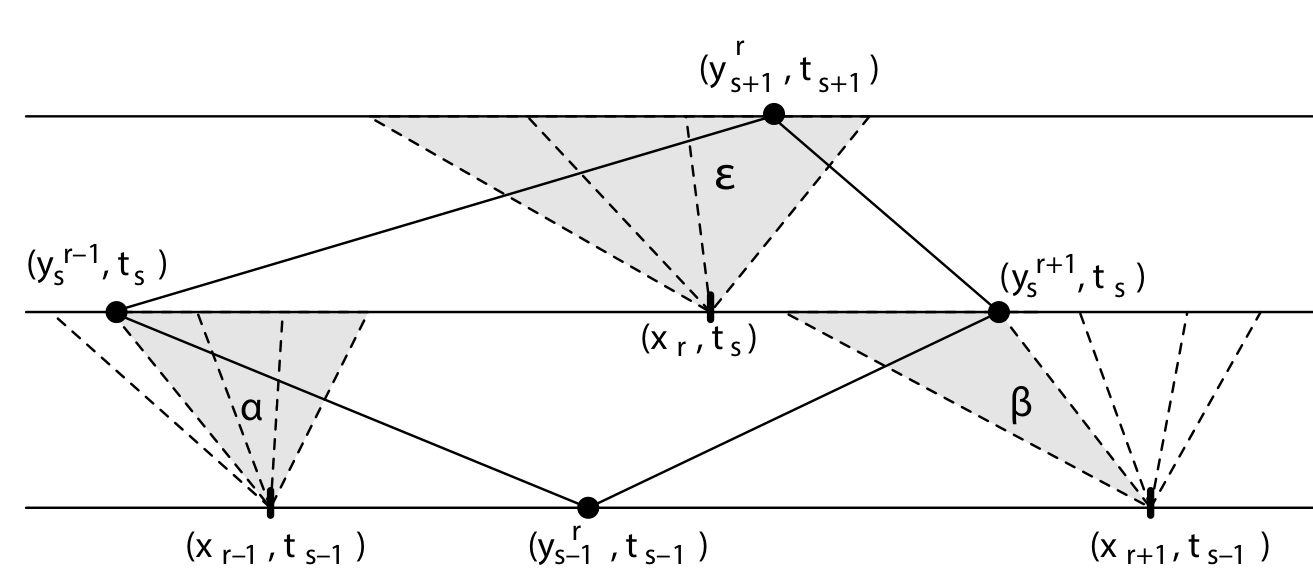
\includegraphics[width=0.9\textwidth]{ch13-fig03-01.png}
\caption{菱形 $\Delta_s^r$ 中的波相互作用：入射波扇 $\alpha,\beta$ 与出射波扇 $\varepsilon$}\label{figure:ch13-菱形相互作用}
\end{figure}

从 $(x_{r-1},t_{s-1})$ 发出、连接左方状态 $U_s^{r-1}$ 与右方状态 $U_{s-1}^r$ 的波扇，通过 $\Delta_s^r$ 的``西南''边进入。如\cref{chapter:ch09-容许波扇与riemann问题}与\cref{chapter:ch09-容许波扇与riemann问题}所解释，
它可用其波振幅的 $n$ 元组 $\alpha=(\alpha_1,\cdots,\alpha_n)$ 表示。第二个波扇从 $(x_{r+1},t_{s-1})$ 发出，连接左方状态 $U_{s-1}^r$ 与右方状态 $U_s^{r+1}$，类似地用波振幅的 $n$ 元组 $\beta=(\beta_1,\cdots,\beta_n)$ 表示，通过 $\Delta_s^r$ 的``东南''边进入。

$\Delta_s^r$ 的输出由从 $(x_r,t_s)$ 发出的完整波扇组成，它连接左方状态 $U_s^{r-1}$ 与右方状态 $U_s^{r+1}$，用其波振幅的 $n$ 元组 $\varepsilon=(\varepsilon_1,\cdots,\varepsilon_n)$ 表示。$\beta$ 的一部分 $\beta'=(\beta_1',\cdots,\beta_n')$ 通过 $\Delta_s^r$ 的``西北''边离开，进入菱形 $\Delta_{s+1}^{r-1}$；而其余部分 $\alpha'=(\alpha_1',\cdots,\alpha_n')$ 通过 $\Delta_s^r$ 的``东北''边离开，进入菱形 $\Delta_{s+1}^{r+1}$。显然 $\varepsilon_i=\alpha_i'+\beta_i'$，$i=1,\cdots,n$。如\cref{chapter:ch09-容许波扇与riemann问题}所解释，
对真非线性特征族，正振幅表示稀疏波，负振幅表示压缩激波。不言而喻，零振幅表示该族的波在所论波扇中缺失。特别地，可确定 $j=1,\cdots,n$，使得当 $i=1,\cdots,j-1$ 时 $\alpha_i'=0$，当 $i=j+1,\cdots,n$ 时 $\beta_i'=0$。$\alpha_j'$ 与 $\beta_j'$ 可同时非零，但此时二者必均为正，对应稀疏波。

若让入射波扇 $\alpha$ 与 $\beta$ 自由传播、越过 $t_s$ 时间线，所产生的波相互作用将生成极为复杂的波型。然而，按\cref{chapter:ch09-容许波扇与riemann问题}中的讨论，
可以预期当 $t\to\infty$ 时该波型将退化为一个中心波扇，即 $\varepsilon$。因此，构造格式的实质在于，用真实的、复杂的波型的时间渐近简化形式来替代它们。在此关联中，``随机选择''的作用是安排波扇的相对位置，使``平均而言''``质量''守恒律成立。

按\cref{chapter:ch09-容许波扇与riemann问题}的术语，
波扇 $\varepsilon$ 应被视为左方波扇 $\alpha$ 与右方波扇 $\beta$ 相互作用的结果。方便起见，把 $\varepsilon,\alpha,\beta$ 实现为赋以 $\ell_1^n$ 范数的 $n$ 维向量，此时\cref{chapter:ch09-容许波扇与riemann问题}给出估计
\begin{align}
|\varepsilon-(\alpha+\beta)|\leqslant[c_3+c_4(|\alpha|+|\beta|)]\mathscr{D}(\Delta_s^r),
\label{align:ch13-int-main}
\end{align}
其中 $c_3,c_4$ 仅依赖于 $F$。特别地，当系统配备 Riemann 不变量坐标系时 $c_3=0$。此处符号 $\mathscr{D}(\Delta_s^r)$ 代替\cref{chapter:ch09-容许波扇与riemann问题}中的 $D(\alpha,\beta)$，
表示菱形 $\Delta_s^r$ 中的波相互作用量，即
\begin{align}
\mathscr{D}(\Delta_s^r)=\sum_{\mathrm{app}}|\alpha_k||\beta_j|.
\label{align:ch13-D-def}
\end{align}
求和遍历所有趋近波对，即所有满足 $k>j$，或 $k=j$ 且 $\alpha_j,\beta_j$ 中至少一个为负（对应激波）的 $(k,j)$。

\eqref{align:ch13-int-main}将用作估计近似解 $U_h$ 的总变差与上确界如何随时间因波相互作用而变化的工具。它足以建立所需的稳定性估计，从而推出算法的收敛性与 Cauchy 问题解的存在性。然而，为研究解的更精细性质，必须更仔细地考察波相互作用，着眼于可能的抵消。

由\eqref{align:ch13-int-main}，当 $\alpha_i$ 与 $\beta_i$ 同号时，离开菱形 $\Delta_s^r$ 的 $i$ 波总强度 $|\alpha_i'|+|\beta_i'|$ 几乎等于入射 $i$ 波的总强度 $|\alpha_i|+|\beta_i|$。然而，当 $\alpha_i$ 与 $\beta_i$ 异号时，$i$ 波发生抵消。为说明这一显著影响解行为的现象，现引入若干概念。菱形 $\Delta_s^r$ 中 $i$ 波的抵消量方便地由下式度量：
\begin{align}
\mathscr{C}_i(\Delta_s^r)=\frac12\big(|\alpha_i|+|\beta_i|-|\alpha_i+\beta_i|\big).
\label{align:ch13-Ci-def}
\end{align}
为分别计及激波与稀疏波，我们把\eqref{align:ch13-int-main}改写为
\begin{align}
\varepsilon_i^{\pm}=\alpha_i^{\pm}+\beta_i^{\pm}-\mathscr{C}_i(\Delta_s^r)+[c_3O(1)+O(\tau)]\mathscr{D}(\Delta_s^r),
\label{align:ch13-int-signed}
\end{align}
其中上标 $+$ 或 $-$ 表示振幅的正部或负部，$\tau$ 是 $U_h$ 的振幅。

把\eqref{align:ch13-int-signed}对任意菱形集合（其并为上半平面中的区域 $\Lambda$）求和，得到方程
\begin{align}
L_i^{\pm}(\Lambda)=E_i^{\pm}(\Lambda)-\mathscr{C}_i(\Lambda)+[c_3O(1)+O(\tau)]\mathscr{D}(\Lambda),
\label{align:ch13-balance}
\end{align}
其中 $E_i^-$（或 $E_i^+$）表示进入 $\Lambda$ 的 $i$ 激波（或 $i$ 稀疏波）总量，$L_i^-$（或 $L_i^+$）表示离开 $\Lambda$ 的 $i$ 激波（或 $i$ 稀疏波）总量，$\mathscr{C}_i(\Lambda)$ 是 $\Lambda$ 内 $i$ 波的抵消量，$\mathscr{D}(\Lambda)$ 是 $\Lambda$ 内的波相互作用量。方程\eqref{align:ch13-balance}表达了 $i$ 波相对于 $\Lambda$ 的平衡，因而被称为 $i$ 激波（负号）或 $i$ 稀疏波（正号）的近似守恒律。

菱形 $\Delta_s^r$ 中波抵消的总量自然度量为
\begin{align}
\mathscr{C}(\Delta_s^r)=\sum_{i=1}^n\mathscr{C}_i(\Delta_s^r).
\label{align:ch13-C-def}
\end{align}
注意到\eqref{align:ch13-int-main}蕴含
\begin{align}
|\alpha'|+|\beta'|=|\varepsilon|\leqslant|\alpha|+|\beta|-2\mathscr{C}(\Delta_s^r)+[c_3+c_4(|\alpha|+|\beta|)]\mathscr{D}(\Delta_s^r).
\label{align:ch13-cancel-est}
\end{align}

\end{document}